\documentclass[12pt, a4paper,twoside,openright]{nufastthesis}
\date{2020} % Year of Thesis Defense
\title{Title} % Title of Thesis
\author{Name} % Candidate Name
\rollno{20K-1234}
\degree{Degree Name} % Doctor of Philosophy or Master of Science or Bachelor of Science
\shortdeg{PhD} % PhD or MS or BS
\printingdate{September 30, 2020} % Thesis Printing Date
\gau{Department of ABC} % Department of Electrical Engineering or Department of Computer Science
\supervisor{Dr. JKL}
\internalexam{Dr. MNO}
\externalexamone{Dr. PQR}
\externalexamoneaffiliation{University of UVW, XYZ}
\externalexamtwo{Dr. DEF}
\externalexamtwoaffiliation{University of GHI, STU}
\city{Karachi} % Peshawar, Islamabad, Lahore, Chiniot-Faisalabad, Karachi

\makeatletter
\let\inserttitle\@title
\let\insertauthor\@author
\let\insertrollno\@rollno
\let\insertdegree\@degree
\let\insertshortdeg\@shortdeg
\let\insertprintingdate\@printingdate
\let\insertgau\@gau
\let\insertsupervisor\@supervisor
\let\insertinternalexam\@internalexam
\let\insertexternalexamone\@externalexamone
\let\insertexternalexamoneaffiliation\@externalexamoneaffiliation
\let\insertexternalexamtwo\@externalexamtwo
\let\insertexternalexamtwoaffiliation\@externalexamtwoaffiliation
\let\insertcity\@city
\makeatother

\makeatletter
\def\cleardoublepage{\clearpage\if@twoside%
\ifodd\c@page\else
\vspace*{8cm}
\begin{center}
This page intentionally left blank.
\end{center}
\thispagestyle{empty}
\newpage
\if@twocolumn\hbox{}\newpage\fi\fi\fi
}
\makeatother

\usepackage{lmodern}\usepackage[T1]{fontenc}
\usepackage{amsmath}
\usepackage{amsthm}
\usepackage[inner=35mm, outer=25mm, top=25mm, bottom=25mm]{geometry}
\usepackage{comment}
\usepackage{fancybox}

\usepackage[fit]{truncate}
\usepackage{fancyhdr}
\fancyhf{}%to clear the page numbering of the fancyhdr package
\addtolength{\headheight}{3pt}
\renewcommand\headrulewidth{0pt}
\fancyhead[R]{\thepage}

\usepackage{listings}
\lstset{% general command to set parameter(s)
basicstyle=\ttfamily\footnotesize,% print whole listing in this sytle
keywordstyle=\color{blue}\bfseries,%\underbar
identifierstyle=,%
commentstyle=\footnotesize,%
stringstyle=\ttfamily,%
showstringspaces=false,%
numbers=left,%none
numberstyle=\ttfamily\footnotesize,%
stepnumber=1,%
numbersep=5pt,%
breaklines=true,breakindent=0pt,%
prebreak=\mbox{\scriptsize$\searrow$},%
postbreak=\mbox{{\color{blue}\scriptsize$\rightarrow$}},%
escapeinside={(*@}{@*)}%
}
%\usepackage[numbers]{natbib}%sort&compress
\usepackage{cite}
\usepackage{notoccite}

\usepackage[dvipsnames]{xcolor}
\definecolor{myblue}{RGB}{54 100 139}%{rgb}{0.2 0.36 0.77}{0 0.2 0.4}{0,0.08,0.45}
\usepackage[font={color=myblue,sf},labelfont=bf,labelsep=period]{caption}
\usepackage[font={small,sf},list=true,labelformat=simple]{subcaption}
\renewcommand\thesubfigure{(\alph{subfigure})} %to include subfig references in ()
% to have the same indention (2.5em) as the subfig package
\makeatletter
\def\l@subfigure{\@dottedtocline{2}{3.8em}{2.5em}}%
\makeatother
\usepackage{psfrag}
\usepackage{setspace}
\usepackage{multicol}
\usepackage{graphicx}
\usepackage{morefloats} %to increase the float queue from 18 floats to 36 floats.  see epslatex.pdf
\graphicspath{{Figures/}}
\usepackage{rotating}
\usepackage{pdflscape}
\usepackage{url}
\interdisplaylinepenalty=2500
\usepackage{array}
\usepackage{tabularx}
\usepackage{tabulary}
\usepackage{longtable}
\usepackage{supertabular}
\usepackage{threeparttable}
\usepackage{booktabs}
\usepackage{placeins}
\usepackage{bm}
\usepackage{lettrine}
\usepackage{tocbibind} %adds toc, lot, lof, bibliography and index to toc.
\usepackage{makeidx}
\makeindex
\usepackage[intoc,refpage,norefeq,prefix]{nomencl}
\setlength{\nomitemsep}{-\parsep}
\makenomenclature
\renewcommand{\nomname}{List of Symbols, Nomenclature or Abbreviations}%The word 'Symbols' is not working in font substitution of Symbol font with StandardSymL
%To make hyperref links (works for page ref only) for nomencl package
\renewcommand*{\pagedeclaration}[1]{\unskip, \hyperpage{#1}}
\usepackage{balance}
\usepackage{appendix}
\usepackage{varioref}

\makeatletter
\renewcommand{\@pnumwidth}{1.75em}
\renewcommand{\@tocrmarg}{2.75em}
\makeatother

\usepackage{hyperref}%
\hypersetup{
final,%
pdfstartview={Fit},%FitH null
pdfpagelayout={SinglePage},%OneColumn
pdfprintscaling={None},%To print the document without shrinking
%pdfborderstyle={/S/U/W 1},% To underline the links
%pdfborderstyle={/S/D/D[3 2]/W 1},% To dash the links
breaklinks=false,%
colorlinks=false,%true
linktoc=page,%all
bookmarksnumbered=true,%
bookmarksopen=false,%
bookmarksopenlevel=2,%
pdfhighlight=/O,%
citebordercolor={0 0 1},%
linkbordercolor={1 0 1},%Magenta
urlbordercolor={0 1 1},%Cyan
citecolor=Black,%Brown
urlcolor=Black,%Cyan
linkcolor=Black,%OliveGreen
pdfauthor={\insertauthor},%
pdfkeywords={},%
pdfsubject={\insertshortdeg{} Thesis},%
pdftitle={\inserttitle}%
}

\usepackage[hyphenbreaks]{breakurl}% to berak long url names in the bibliography
\usepackage[hyperpageref]{backref} % to be loaded after hyperref package
\renewcommand*{\backref}[1]{}  % Disable standard
\renewcommand*{\backrefalt}[4]{% Detailed backref
\ifcase #1 %
\relax%(Not cited.)%
\or
(cited on page~#2.)%
\else
(cited on pages~#2.)
\fi}

\setcounter{topnumber}{4}
\setcounter{bottomnumber}{4}
\setcounter{totalnumber}{10}
\renewcommand{\textfraction}{0.15}
\renewcommand{\topfraction}{0.85}
\renewcommand{\bottomfraction}{0.70}
\renewcommand{\floatpagefraction}{0.66}
\setlength{\floatsep}{5pt plus 3pt minus 2pt}
\setlength{\textfloatsep}{12pt plus 2pt minus 4pt}

%to balance the columns on the last page of index
% taken from http://www.scribd.com/doc/2633955/Writing-a-thesis-with-LaTeX
\let\orgtheindex\theindex
\let\orgendtheindex\endtheindex
\def\theindex{%
\def\twocolumn{\begin{multicols}{2}}%
\def\onecolumn{}%
\clearpage
\orgtheindex
}
\def\endtheindex{%
\end{multicols}%
\orgendtheindex
}

\begin{document}
\pdfbookmark[0]{Title Page}{chap:titlepage} % to add pdf bookmark
\nufasttitlepage
\setcounter{secnumdepth}{3} \setcounter{tocdepth}{2}
\pagestyle{empty}
\pagenumbering{roman}
%%-----------Plagiarism Undertaking---------------
\chapter*{Plagiarism Undertaking}
\pdfbookmark[0]{Plagiarism Undertaking}{chap:plagiarism_undertaking} % to add pdf bookmark
%\addcontentsline{toc}{chapter}{Plagiarism Undertaking}
\setcounter{page}{1}
\thispagestyle{empty}

I take full responsibility of the research work conducted during the \insertshortdeg{} Thesis titled \inserttitle. I solemnly declare that the research work presented in the thesis is done solely by me with no significant help from any other person; however, small help wherever taken is duly acknowledged. I have also written the complete thesis by myself. Moreover, I have not presented this thesis (or substantially similar research work) or any part of the thesis previously to any other degree awarding institution within Pakistan or abroad.

I understand that the management of National University of Computer and Emerging Sciences has a zero tolerance policy towards plagiarism. Therefore, I as an author of the above-mentioned thesis, solemnly declare that no portion of my thesis has been plagiarized and any material used in the thesis from other sources is properly referenced. Moreover, the thesis does not contain any literal citing of more than 70 words (total) even by giving a reference unless I have the written permission of the publisher to do so. Furthermore, the work presented in the thesis is my own original work and I have positively cited the related work of the other researchers by clearly differentiating my work from their relevant work.

I further understand that if I am found guilty of any form of plagiarism in my thesis work even after my graduation, the University reserves the right to revoke my \insertshortdeg{} degree. Moreover, the University will also have the right to publish my name on its website that keeps a record of the students who plagiarized in their thesis work.

\vskip 3em
$\overline{\text{\insertauthor}}$

Date: \insertprintingdate
%%-----------Author's Declaration---------------
\chapter*{Author's Declaration}
\pdfbookmark[0]{Author's Declaration}{chap:author_declaration} % to add pdf bookmark
%\addcontentsline{toc}{chapter}{Author's Declaration}
\thispagestyle{empty}

I, \insertauthor, hereby state that my \insertshortdeg{} thesis titled \inserttitle{} is my own work and it has not been previously submitted by me for taking partial or full credit for the award of any degree at this University or anywhere else in the world. If my statement is found to be incorrect, at any time even after my graduation, the University has the right to revoke my \insertshortdeg{} degree.

\vskip 3em
$\overline{\text{\insertauthor}}$

Date: \insertprintingdate
\cleardoublepage
%%-----------Certificate of Approval---------------
%\chapter*{Certificate of Approval}
\pdfbookmark[0]{Certificate of Approval}{chap:certificate_of_approval} % to add pdf bookmark
%\addcontentsline{toc}{chapter}{Certificate of Approval}
\vspace*{4em}
\begin{center}
\textbf{\LARGE Certificate of Approval}

\vskip 4em
\itshape
\noindent It is certified that the research work presented in this thesis, entitled ``\inserttitle'' was conducted by \insertauthor{} under the supervision of \insertsupervisor.

\vskip 0.5em
\noindent No part of this thesis has been submitted anywhere else for any other degree.

\vskip 0.5em
\noindent This thesis is submitted to the \insertgau{} in partial fulfillment of the requirements for the degree of \insertdegree{} in ``\insertgau'' at the \insertcity{} campus of

\vskip 0.5em
\noindent National University of Computer and Emerging Sciences, Islamabad, Pakistan.

\vskip 0.5em
\insertprintingdate
\end{center}

\vskip 1em
\noindent\begin{tabular}{p{1.5in}p{2in}ll}
Candidate Name: & \underline{\insertauthor} & Signature: & \makebox[1in]{\hrulefill}
\end{tabular}

\vskip 3em
\noindent\textbf{Examination Committee:}

\vskip 2em
\noindent\begin{tabular}{p{1.5in}p{2in}ll}
External Examiner 1: & \underline{\insertexternalexamone} & Signature: & \makebox[1in]{\hrulefill}\\[1em]
&\multicolumn{3}{p{4in}}{\underline{\insertexternalexamoneaffiliation}}\\[3em]
External Examiner 2: & \underline{\insertexternalexamtwo} & Signature: & \makebox[1in]{\hrulefill}\\[1em]
&\multicolumn{3}{p{4in}}{\underline{\insertexternalexamtwoaffiliation}}\\[3em]
Internal Examiner: & \underline{\insertinternalexam} & Signature: & \makebox[1in]{\hrulefill}
\end{tabular}

\vskip 3em
\noindent\textbf{Supervisor:}

\vskip 2em
\noindent\begin{tabular}{p{1.5in}p{2in}ll}
Supervisor: & \underline{\insertsupervisor} & Signature: & \makebox[1in]{\hrulefill}
\end{tabular}
\cleardoublepage
%% -----------Dedication----------------
%\chapter*{Dedication}
\pdfbookmark[0]{Dedication}{chap:dedication} % to add pdf bookmark
%\addcontentsline{toc}{chapter}{Dedication}
%\thisfancyput*(2.5in,-1.5in){
\includegraphics[width=2in]{Bismillah}}
\begin{center}
\null\vspace{\stretch{1}}
{\usefont{T1}{pzc}{m}{n}\selectfont\large Dedicated to My parents and Family.}
\vspace{\stretch{2}}\null
\end{center}
%%-------------Abstract-----------------
\doublespacing
\chapter*{Abstract}
\pdfbookmark[0]{Abstract}{chap:abstract} % to add pdf bookmark
%\addcontentsline{toc}{chapter}{Abstract}
\thispagestyle{empty}

Start writing from here.
(not more than 500 words).

%%-----------Acknowledgements---------------
\chapter*{Acknowledgements}
\pdfbookmark[0]{Acknowledgements}{chap:acknowledgements} % to add pdf bookmark
%\addcontentsline{toc}{chapter}{Acknowledgements}
\thispagestyle{empty}

I would like to express my sincere gratitude to my supervisor \insertsupervisor{} for suggesting the topic, his guidance and continuous support.  This work would not have been successful without his previous research, full encouragement and valuable advice.

Above all, I would like to thank my parents and my family for their love, support and patience throughout the duration of my thesis work.
\cleardoublepage
\pagestyle{plain}
%%-----------Table of Contents------------------
\tableofcontents
%%------------List of Tables----------------------
\listoftables
%%------------List of Figures----------------------
\listoffigures
\printnomenclature[1.25in]
\cleardoublepage
%to make cite border of correct height
\makeatletter\let\org@hyper@linkend\hyper@linkend\def\hyper@linkend{\baselineskip=0.5\baselineskip\org@hyper@linkend}\makeatother
\pagenumbering{arabic}
\fancyhf{}
\fancyfoot[C]{\thepage}
\pagestyle{fancy}
%%-----------Chapters start-------------------------------------
%%-----------Chapter 1------------------------------------------
\chapter{Introduction}


Session-based recommendation is a very common recommendation problem that is encountered in many domains such as e-commerce, classified sites, music and video recommendation. In the session-based setting, past user history logs are typically not available (either because the user is new or not logged-in or not tracked) and recommend-er systems have to rely only on the actions of the user in the current sessions to provide accurate recommendations. Until recently many of these recommendations tasks were tackled mainly using relatively simple methods such as item-based collaborative filtering \cite{sarwar2001item} or content-based methods. Recurrent Neural Networks (RNNs)\nomenclature{RNN}{Recurrent Neural Network} have emerged from the deep learning literature as powerful methods for modeling sequential data. These models have been successfully applied in speech recognition, translation, time series fore casting and signal processing. In recommend er systems RNNs have been recently applied to the session-based recommendation setting with impressive results \cite{hidasi2012fast}. 

\label{chap:introduction}
\section{Traditional History}
The advantage of RNNs over traditional similarity-based methods for recommendation is that they can effectively model the whole session of user interactions (clicks, views, etc.). By modeling the whole session RNNs can in effect learn the ‘theme’ of the session and thus provide recommendations with increased accuracy (between 20\%-30\%) over traditional methods.

RNNs in session-based recommendation have been adapted to the task of recommendation. One of the main objectives in recommendation is to rank items by user preference; i.e. the exact ranking or scoring of items in the tail of the item list (items that the user will not like) is not that important, but it is very important to rank correctly the items that the user will like at the top of the list (first 5, 10 or 20 positions). To achieve this with machine learning one has to typically utilize learning to rank techniques(see e.g. \cite{burges2010ranknet}) and in particular ranking objectives and loss functions. The current session-based RNN approaches use ranking loss functions and, in particular, pairwise ranking loss functions. As in most deep learning approaches the choice of a good ranking loss can have a very significant influence on performance. Since deep learning methods need to propagate gradients over several layers and in the case of RNNs’back in time’over previous steps,to optimize the model parameters, the quality of these gradients originating from the loss function influences the quality of the optimization and the model parameters. Moreover the nature of the recommendation task, which typically entails large output spaces (due to large number of items), poses unique challenges that have to be taken in to account as well when designing a proper ranking loss function. We will see that the way this large output space issue is tackled is very crucial in achieving good performance.







\label{sec:abc}
\subsection{How Impact our loss function}

In this work we analyze ranking loss functions used in RNNs for session-based recommendations, this analysis leads to a new set of ranking loss functions that increase the performance of the RNN upto 30\% over previous commonly used losses without incurring in significant computational overheads. We essentially devise a new class of loss functions that combines learnings from the deep learning and the learning to rank literature. Experimental results on several datasets coming from industry validate these impressive improvements,in terms of Mean Reciprocal Rank(MRR)\nomenclature{MRP}{Mean Reciprocal} and Recall@20. With these improvements the difference between RNNs and conventional memory-based collaborative filtering jumps to 51\% in terms of MRR and Recall@20 demonstrating the potential that deep learning methods bring to the area of Recommender Systems. NU.  It is also known as FAST\index{FAST}. \nomenclature{PK}{Pakistan}
\index{PK}

\subsection{RELATED WORK}
One of the main approaches that is employed in session-based recommendation and a natural solution to the problem of a missing user profile is the item-to-item recommendation approach \cite{sarwar2001item}. In this setting, an item-to-item similarity matrix is precomputed from the available session data, that is items that are often clicked together in sessions are deemed to be similar. This similarity matrix is then simply used during the session to recommend the most similar items to the one the user has currently clicked. 

Long Short-Term Memory(LSTM) \cite{hochreiter1997long} networks area type of RNNs that have been shown to solve the optimization issues the plague vanilla-type RNNs. LSTM’s include additional gates that regulate when and how much of the input to take into account and when to reset the hidden state. As lightly simplified version of LSTM–that still maintains all their properties – are Gated Recurrent Units (GRUs) \cite{cho2014bv}, which we use in this work. Recurrent Neural Networks have been used with success in the area of session-based recommendations; \cite{hidasi2016a} proposed a Recurrent Neural Network with a pairwise ranking loss for this task, \cite{tan2016improved} proposed data augmentation techniques to improve the performance of the RNN for session-based recommendations; these techniques have though the side effect of increasing training times as a single session is split into several sub-sessions for training. Session-based RNNs have been augmented \cite{hidasi2016parallel} b with feature information, such as text and images from the clicked/consumed items, showing improved performance over the plain models. RNNs have also been used in more standard user-item collaborative filtering settings where the aim is to model the evolution of the user and items factors \cite{wu2017recurrent},\cite{devooght2016collaborative} where the results are less striking, with the proposed methods barely outperforming standard matrix factorization methods. This is to be expected as there is no strong evidence on major user taste evolution in a single domain in the time frames of the available datasets and sequential modeling of items that are not ’consumed’ in sessions such as movies might not bring major benefits. 

Another area touched upon in this work are loss functions tailored to recommender systems requirements. This typically means ranking loss functions. In this area there has been work particularly in
the context of matrix factorization techniques. One of the first learning to rank techniques for collaborative filtering was introduced in \cite{weimer2007cofirank}. Essentially a listwise loss function was
introduced along with an alternating bundle method for optimization of the factors. Further ranking
loss function for collaborative filtering were introduced in \cite{shi2012climf} \cite{rendle2012bpr}
and \cite{rendle2012bpr}. Note that the fact that these loss functions work well in matrix factorization does not guarantee in any way that they are an optimal choice for RNNs as back propagation
requirements are stronger than those posed by simple SGD. We will in fact see that BPR, a popular
choice of loss function, needs to be significantly modified to extract optimal results in the case of
RNNs for session-based recommendations. Another work related to sampling large output spaces
in deep networks for efficient loss computations for language models is the ’blackout’ method \cite{ji2015blackout}, where essentially a sampling procedure similar to the one used in \cite{hidasi2015session}
is applied in order to efficiently compute the categorical cross-entropy loss.


%% Please note that we have introduced automatic line number generation
%% into the style file for \LaTeXe. This is to help reviewers
%% refer to specific lines of the paper when they make their comments. Please do
%% NOT refer to these line numbers in your paper as they will be removed from the
%% style file for the final version of accepted papers.



%%----------Chapter 2------------------------------------------
\chapter{Literature Review}
\section{Example Citation}
%%---------------example citation---------------------
Start writing from here. Here is a citation~\cite{Knuth92}.
\section{Example Tables}
\subsection{A Table With Border}
Exam results are given in Table~\ref{tab:Results}.
%%------------------example table--------------------
\begin{table}[htbp]
\caption{Example table}
\label{tab:Results}
\begin{center}
\begin{tabular}{| l || r | r | r | c |}
\hline
Name&Exam1&Exam2&Exam3&Grade\\
\hline\hline
Ahmed&19& 28&33&C \\
\hline
Daud&49& 35&60&B  \\
\hline
Zain&76& 38&59&A  \\
\hline
\end{tabular}
\end{center}
\end{table}

\subsection{A Table Without Border}
Table~\ref{tab:MathSymbols} is an example table without borders.  Some symbols with label can be refereed later on.
\begin{table}[htbp]
\caption{Variable-sized  Symbols}
\label{tab:MathSymbols}
\begin{center}
\begin{tabular}{l l l l l l}
$\sum$  \label{p1}&$\backslash$sum   &$\bigcap$ \label{p2}&$\backslash$bigcap      &$\bigodot$   &$\backslash$bigodot  \\
$\prod$ &$\backslash$prod  &$\bigcup$   &$\backslash$bigcup    &$\bigotimes$ &$\backslash$bigotimes\\
$\coprod$ &$\backslash$coprod &$\bigsqcup$ &$\backslash$bigsqcup  &$\bigoplus$ &$\backslash$bigoplus \\
$\int$     &$\backslash$int   &$\bigvee$   &$\backslash$bigvee    &$\biguplus$ &$\backslash$biguplus\\
$\oint$     &$\backslash$oint &$\bigwedge$ &$\backslash$bigwedge
\end{tabular}
\end{center}
\end{table}

\section{Example List}
\subsection{Example Dotted List}
%%-----------------example dotted list--------------------
\smallskip
\textbf{Some special characters in TeX:}
\begin{itemize}
\item Accents
\item Braces
\item Dollar signs
\end{itemize}

\subsection{Example Numbered List}
%%----------------example numbered list---------------------
\smallskip
\textbf{Some special characters in TeX:}
\begin{enumerate}
\item Accents
\item Braces
\item Dollar signs
\end{enumerate}

\section{Math Example}
\subsection{Inline Math Mode}
%%-------------------example math equation----------
Mathematical material to be typeset inline must be surrounded by a
single dollar sign. For example: $a^2 + b^2 = c^2$.
\subsection{Displayed Math}
This is a displayed math example without numbering.
\[
\lim_{x \to a}f(x)
\]

\[
\left|\sum_{i=1}^n a_ib_i\right| \le \left(\sum_{i=1}^n
a_i^2\right)^{1/2} \left(\sum_{i=1}^n b_i^2\right)^{1/2}
\]

This is a math equation with numbering.
\begin{equation}
(a+b)^3 = (a+b)^2(a+b)
\end{equation}

%%-----------------example aligned equation------------------
This is multiline equation example.
\begin{align}
(a+b)^3 &= (a+b)^2(a+b)\\
&=(a^2+2ab+b^2)(a+b)\\
&=(a^3+2a^2b+ab^2) + (a^2b+2ab^2+b^3)\\
&=a^3+3a^2b+3ab^2+b^3
\end{align}

%%--------------example matrix-------------------------------
This is a matrix
\[
\begin{matrix}
    a+b & uv & x-y & 5\\
    a+b+c & u+v &x+y & 10
\end{matrix}
\]

%%------------example cases----------------------------------
This is a case
\[
f(x)=
\begin{cases}
    -x^{2}, &\text{if $x<0$;}\\
    \alpha+x, &\text{if $0 \leq x \leq 1$;}\\
    x^{2}, &\text{otherwise.}
\end{cases}
\]

%%--------------------example figure-------------------
\section{Graphics Example}
\subsection{Stars}
The ideal graphics format for inclusion in a \LaTeX document is
"encapsulated postscript" or eps. Here is an example figure.
\begin{figure}[htbp]
\begin{center}

\includegraphics[width=\textwidth]{Stars}
\caption{Stars}
\end{center}
\end{figure}
%%--------------------Chapter 3------------------------
\chapter{Methodology}
\section{A Section}
%%--------------------example citation-----------------
Start writing from here~\cite{ConcreteMath}.

\subsection{A Subsection}
some text with footnote\footnote{A first}. more
text\footnote{second} and more.

%%-----------------text superscript, subscript--------------------
A sentence with superscript.\textsuperscript{superscript}. A
sentence with subscript.$_{\mbox{\footnotesize{subscript}}}$

%%-----------------printing verbatim--------------------------------
\subsection{Printing Verbatim}
\begin{verbatim}
THIS TEXT WILL BE DIRECTLY PRINTED AS IF TYPED ON A TYPEWRITER, WITH
ALL LINE BREAKS AND SPACES,              without any LaTex command
being executed.

public class BasicsDemo{
    public static void main(String[] args){
        int sum = 0;
        for (int current = 1; current <= 10; current++){
            sum += current;
        }
        System.out.println("Sum = " + sum);
    }
}
\end{verbatim}

\begin{Verbatim}[frame=single, xrightmargin=2pc]
public class BasicsDemo{
    public static void main(String[] args){
        int sum = 0;
        for (int current = 1; current <= 10; current++){
            sum += current;
        }
        System.out.println("Sum = " + sum);
    }
}
\end{Verbatim}

%%---------------program code-------------------------------------
\section{A Section}
\subsection{Pretty-printing Program Code}
%\begin{algorithmic}
%\IF {$i\leq0$} \STATE $i\gets1$ \ELSE \IF {$i\geq0$} \STATE
%$i\gets0$ \ENDIF \ENDIF
%\end{algorithmic}
\subsubsection{Example Java Code}
The following is an code example:
\begin{lstlisting}[language=Java]
public class BasicsDemo{
    public static void main(String[] args){
        int sum = 0;
        for (int current = 1; current <= 10; current++){
            sum += current;
        }
        System.out.println("Sum = " + sum);
    }
}
\end{lstlisting}
%%-----------------Chapter 4---------------------------
\chapter{LOSS FUNCTION DESIGN}

\label{sec:loss}
In this section we examine the loss functions implemented in GRU4Rec and identify their weaknesses. We propose two ways to stabilize the numerical instability of the cross-entropy loss, we show how learning with the TOP1 and BPR pairwise losses degrades as we add more samples to the
output, and propose a family of loss functions based on pairwise losses that alleviates this problem.
We note that, while our aim is to improve GRU4Rec, the loss functions proposed in this section can
be also used with other models, such as matrix factorization.

\subsection{ CATEGORICAL CROSS-ENTROPY}
Categorical cross-entropy measures the distance of a proposed (discrete) probability distribution q
from the target distribution p as defined by (\ref{eq:1}).

\begin{equation}\label{eq:1}
   H(p,q)=-\sum_{j=1}^{N} p_j  \log\ q_j
\end{equation}

This loss is often used in machine learning and deep learning in particular for multi-class classification problems. Next item recommendation can be interpreted as classification, where the class labels are the items in the system and item sequences need to be assigned with the label of the item that follows. In a single-label scenario – such as next item recommendation – the target distribution is a one-hot vector over the set of items, with the coordinate corresponding to the target item set
to 1. The proposed distribution consists of the scores assigned to the items by the algorithm. The output scores need to be transformed to form a distribution. It is common practice to use the soft max transformation (\ref{eq:2}), which is a continuous approximation of the max operation. This naturally aligns
with the sentiment that the label with the highest score is assigned to the sequence.
\begin{equation}\label{eq:2}
    s_i = \frac{\ e^{r_i} }{\sum_{j=1}^{N} \\ e^{r_i}}
\end{equation}

Cross-entropy in itself is a point wise loss, (that is it can be computed per individual item) as it is the sum of independent losses defined over the coordinates. Combining it with soft max introduces
list wise properties into the loss, since the loss now cannot be separated over coordinates (or items). Putting them together we get the following loss function over the scores (assuming that the target
item is indexed by $i$):

\begin{equation}\label{eq:3}
    L_{xe} = - \log s_i = \frac{\ e^{r_i} }{\sum_{j=1}^{N} \\ e^{r_i}}
\end{equation}

\textbf{Fixing the instability:} One of the losses available in GRU4Rec was cross-entropy with soft max scores. \cite{hidasi2016a} reported slightly better results than with other losses, but deemed the loss to be unstable for a large fraction of the hyper parameter space and thus advised against its use. This instability comes from the limited numerical precision. Assuming that there is a $k$ for which $r_k \gg  r_i , s_i$ becomes very small and rounded to 0, because of the limited precision. The loss
then computes $log \ 0$, which is undefined. Two ways to circumvent this problem are as follow: (a)
compute $− log(s_i +\epsilon)$, where $\epsilon$ is a very small value (we use $10^−24$ ); (b) compute $− log s_i$ directly as $−r _+log \sum_{j=1}^{N} e^{ r^j }. $The former introduces some noise, while the latter does not allow the separated use of the transformation and the loss, but both methods stabilize the loss. We did not observe any differences in the results of the two variants.

\subsubsection{RANKING LOSSES : TOP1 & BPR}
GRU4Rec offers two loss functions based on pairwise losses. Pairwise losses compare the score of the target to a negative example (i.e. any item other than the target). The loss is high if the target’s score is higher than that of the negative example. GRU4Rec computes scores for multiple negative samples per each target, and thus the loss function is composed as the average of the individual
pairwise losses. This results in a list wise loss function, which is composed of pairwise losses.

One of the loss functions is coined TOP1 (\ref{eq:4}). It is a heuristically put together loss consisting of two
parts. The first part aims to push the target score above the score of the samples, while the second
part lowers the score of negative samples towards zero. The latter acts as a regularizer, but instead
of constraining the model weights directly, it penalizes high scores on the negative examples. Since
all items act as a negative score in one training example or another, it generally pushes the scores
down.

\begin{equation}\label{eq:4}
    L_{top1} =  \frac{1}{N_s}  \sum_{j=1}^{N_s} \alpha (r_j - r_i) + \alpha (r^{2}_{j})
\end{equation}

$j$ runs over the ($N_S$ ) sampled negative (’non-relevant’) items, relevant items are index by i. The other loss function (\ref{eq:5}) is based on the popular Bayesian Personalized Ranking (BPR) \cite{rendle2012bpr} loss. Here the negative log-probability of the target score exceeding the sample scores is minimized (i.e. the probability of target scores being above sample scores is maximized). The non-continuous $P (r_i > r_j )$ is approximated by $\alpha(r_i − r_j ).$

\begin{equation}\label{eq:5}
    L_{top1} =  \frac{1}{N_s}  \sum_{j=1}^{N_s} \log \alpha(r_i - r_j)
\end{equation}


\subsubsection{VANISHING GRADIENTS}
Taking the average of individual pairwise losses has an undesired side effect. Examining the gradients for the TOP1 and BPR losses w.r.t. the target score $r_i$, ((6) and (7) respectively) reveals that
under certain circumstances gradients vanish and thus learning stops. With pairwise losses, one
generally wants to have negative samples with high scores, as those samples produce high gradients.
Or intuitively, if the score of the negative sample is already well below that of the target, there is
nothing to learn from that negative sample anymore. For this discussion we will denote samples
where $rj \gg ri$
irrelevant. For an irrelevant sample $\alpha(r_j − r_i)$ in ((6) and $1 − \alpha(r_i − r_j )$ (7) will be close to zero. Therefore, any irrelevant sample adds basically nothing to the total gradient.
Meanwhile the gradient is always discounted by the total number of negative samples. By increasing the number of samples, the number of irrelevant samples increases faster than that of including
relevant samples, since the majority of items is irrelevant as a negative sample. This is especially
true for non-popularity-based sampling and high sample numbers. Therefore these losses start to
vanish as the number of samples increase, which is counter intuitive and hurts the full potential of
the algorithm.\footnote[5]{Simply removing the discounting factor does not solve this problem, since it is equivalent of multiplying the learning rate by $N_S$. This would destabilize learning due to introducing high variance into the updates.}\footnote[6]{For BPR, there is the option of maximizing the sum of individual pairwise probabilities $\sum_{N_S}^{j=1}  P(r_i > r_j )$, \\
i.e. minimizing $− \log \sum_{N_S}^{j=1} \ \alpha(r_i − r_j )$. However, this loss has even worse properties.
}

\begin{equation}\label{eq:6}
    \frac{\partial L_{top^1}}{\partial r_i} = - \frac{1}{N_s} \sigma (r_j - r_i) (1 - \sigma (r_j - r_i))
\end{equation}

\begin{equation}\label{eq:7}
    \frac{\partial L_{bpr}}{\partial r_i} = - \frac{1}{N_s} \sum_{j=1}^{N_S} (1 - \sigma (r_i - r_j)  )
\end{equation}

\graphicspath{{img/}}

\begin{figure}[htp]
    \centering
    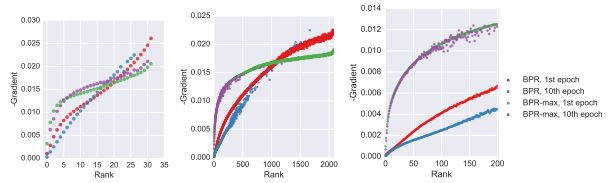
\includegraphics[width=400]{p2}
    \caption{Median negative gradients of BPR and BPR-max w.r.t. the target score against the rank of the target item. Left: only mini batch samples are used (mini batch size: 32); Center: 2048 additional negative samples were added to the mini batch samples; Right: same setting as the center, focusing on ranks 0-200.}
    \label{fig:galaxy}
\end{figure}

\subsection{ RANKING-MAX LOSS FUNCTION FAMILY}
To overcome the vanishing of gradients as the number of samples increase, we propose a new family of listwise loss functions, based on individual pairwise losses. The idea is to have the target score compared with the most relevant sample score, which is the maximal score amongst the samples.

\begin{equation}\label{eq:8}
    L_{pairwise-max}\left ( r_i,\begin{Bmatrix}
r_i
\end{Bmatrix}_{j=1}^{N_S} \right ) = L_[pairwise]\left ( r_i,  \underset{j}{max} \ r_i\right )
\end{equation}
The maximum selection is non-differentiable and thus cannot be used with gradient descent. Therefore we use the softmax scores to preserve differentiability. Here, the soft max transformation is
only used on the negative examples (i.e. $r_i$ is excluded), since we are looking from the maximum score amongst the negative examples. This naturally results in loss functions where each negative sample is taken into account proportional to its likelihood of having the maximal score. Based on this general idea, we now derive the TOP1-max and BPR-max loss functions.

\textbf{TOP1-max} : The TOP1-max loss is fairly straightforward. The regularizing part does not necessarily need to be only applied for the maximal negative score, however we found that this gave the
best results, thus kept it this way. The continuous approximation to the maximum selection entails
summing over the individual losses weighted by the corresponding softmax scores sj , giving us the
TOP1-max loss (\ref{eq:9}).

\ref{eq:9}.

\begin{equation}\label{eq:9}
    L_{top1 - max}\left ( r_i,\begin{Bmatrix}
r_i
\end{Bmatrix}_{j=1}^{N_S} \right )= \sum_{j=1}^{N_S} s_j \left ( \sigma (r_j - r_i) + \sigma (r^2_j) \right )
\end{equation}


The gradient of TOP1-max (\ref{eq:10}) is the sof tmax weighted average \footnote[7]{$\sum s_j = 1$} of individual pairwise gradients.
If $r_j$ is much lower than the maximum of negative scores, its weight will be almost zero and more
weight will be placed on examples with scores close to the maximum. This solves the issue of
vanishing gradients with more samples, because irrelevant samples will be just ignored, while the
gradient will point towards the gradient of the relevant samples. Of course, if all samples are irrelevant, the gradient becomes near zero, but this is not a problem, since if the target score is greater
than all sample scores, there is nothing to be learned. Unfortunately, the sensitivity to large sample
scores of TOP1 is still an issue as it is the consequence of the pairwise loss and not the aggregation


\begin{equation}\label{eq:10}
  \frac{\partial L_{top^1 - max}}{\partial r_i} = \sum_{j=1}^{N_S} s_j\sigma(r_j - r_i)(1 - \sigma(r_j - r_i))
  \end{equation}



\textbf{BPR-max:} Going back to the probability interpretation of BPR, the goal is to maximize the probability of the target score being higher than the maximal sample score $r_max = max_j r_j$ . This can be
rewritten using conditional probabilities:

\begin{equation}\label{eq:11}
  p\left ( r_i  > r_{max} \right ) = \sum_{j=1}^{N_S} P\left ( r_i > r_j | r_j = r_{max} \right ) P (r_j = r_{max})
  \end{equation}



$P(r_i > r_j )$ and $P(r_j = r_{max})$ is approximated by $\sigma(r_i − r_j )$ (as in the original BPR loss) and the
softmax score $s_j$ respectively. We then want to minimize the negative log-probability, which gives
us the loss

\begin{equation}\label{eq:12}
  L_{bpr-max} = \log \sum_{j=1}^{N_S} s_j \sigma (r_i - r_j)
  \end{equation}


The gradient of BPR-max (\ref{eq:13}) is the weighted average of individual BPR gradients, where the
weights are $s_j \sigma (r_i − r_j)$. The relative importance of negative samples $j$ and $k$ is 
$\frac{\sigma(ri−rj )s_j} {\sigma(r_i−r_k)s_k} = \frac{e^r_j + e^{-r_i+rj+r_k}}{e^rk + e^{-r_i+r_j+r_k}} $
, which behaves like softmax weights if $ri \gg rj + rk$ or if both ri and rk are small.
Otherwise it is a smoothed softmax. This means that while $r_i$is small, the weights are distributed
more evenly, yet clear emphasis will be given to higher sample scores. As $r_i$ becomes higher, the
focus shifts quickly to the samples with high scores. This is an ideal behaviour

\begin{equation}\label{eq:13}
  \frac{\partial L_{bpr-max}} {\partial r_i} = - \frac{\sum_{j=1}^{N_S} s_j \sigma(r_i - r_j)(1-\sigma (r_i - r_j))} {\sum_{j=1}^{N_S} s_j \sigma (r_i - r_j)}
\end{equation}

The gradient w.r.t. a negative sample – with both the BPR-max and TOP1-max – is proportional to the softmax score of the example, meaning that only the items, near the maximum will be updated. This is beneficial, because if the score of a negative sample is low, it doesn’t need to be updated. If the score of a sample is much higher than that of the others it will be the only one updated and the gradient will coincide with the gradient of the pairwise loss between the target and the sample score. In a more balanced setting the gradient is between the aforementioned gradient and 0. For example the gradient of BPR-max w.r.t. a negative sample’s score is as follows:


\begin{equation}\label{eq:14}
  \frac{\partial L_{bpr-max}} {\partial r_k} = S_K - \frac{S_K \alpha^2 (r_i - r_K)} {\sum_{j=1}^{N_S} s_j \sigma (r_i - r_j)}
\end{equation}

Figure 2 depicts how the gradients of BPR and BPR-max behave given the rank of the target item \footnote[8]{Similar trends can be observed when comparing TOP1 and TOP1-max, even though the shape of the curves
is quite different from that of BPR.}.
The rank of the target is the number of negative scores exceeding it, e.g. rank 0 means that the target score is higher than all sample scores. Lower rank means that there are fewer negative samples that are relevant. The figure depicts the median negative gradient w.r.t. the target score in two cases, measured on a dataset sample during the $1^st$ and $10^th$ epochs (i.e. beginning and end of the training): (left) no additional samples were used, only the other examples from a mini-batch of size 32; (middle & right) 2048 additional negative samples were added. The rightmost figure focuses on the first 200 ranks of the figure in the middle. The gradient is slightly higher for BPR when there are more relevant samples (i.e. high ranks). This is natural, since BPR-max focuses on samples closest to the maximum value and ignores other still relevant samples. This entails slightly slower learning for BPR-max when the target item is ranked at the end of the list, but the difference is not really significant. On the other hand, the gradient of BPR quickly vanishes as the number of relevant samples decrease (i.e. low ranks). The point of vanishing is relative to the total sample size. With small sample size, BPR’s gradient starts vanishing around rank 5 (the BPR-max does not vanish until rank 0); meanwhile, with more samples, the BPR gradient is very low, even for rank 100-500 (again, the gradient BPR-max starts decreasing significantly later). This means that BPR can hardly push target scores up in the ranking after a certain point, which comes earlier as the number of sample size increases. BPR-max, on the other hand, behaves well and is able to improve the score all the way.

\subsubsection{ BPR-MAX WITH SCORE REGULARIZATION}

Even though we showed that the heuristic TOP1 loss is sensitive to relevant samples with very high scores, it was found to be performing better than BPR in \cite{hidasi2016a}. According to our observation, the same is true for the relation of TOP1-max and BPR-max. Part of the reasons lies in the rare occurrence of $r_j \gg r_i$ while $r_j ≈ 0$ simultaneously. If only the first condition is met, the gradient w.r.t. $r_i$ might vanish, but the regularizing part of TOP1 makes sure that $r_j$ is moved towards zero, which might even make the update possible for $r_i$ next time (e.g. if $r_j$ was negative, moving it towards zero decreases the difference with ri). The score regularization in TOP1 is very beneficial to the overall learning process, so even though the loss might not be theoretically optimal,it can achieve good results. GRU4Rec support two forms of regularization with every loss: dropout and $l_2$ regularization of the model parameters. The regularization of TOP1 is used on the top of these. According to our experiments, the $2$ regularization of model parameters decreases the model performance. Our assumption is that some of the model weights – such as the weight matrices for computing the update and reset gate – should not be regularized. Penalizing high output scores takes care of constraining the model, even without explicitly regularizing the weights.


Therefore we added score regularization to the BPR-max loss function as well. We tried several ways of score regularization. In the best performing one we conditioned the sample scores on
independent, zero mean Gaussians with variance inversely proportional to the softmax score (\ref{eq:15}).This entails stronger regularization on scores closer to the maximum, which is ideal in our case.

\begin{equation}\label{eq:15}
P(r_i > r_{max}|\begin{Bmatrix}
r_j
\end{Bmatrix}_{j=1}^{N_S})\prod_{j=1}^{N_S} P(r_j) = P (r_i > r_{max}| \begin{Bmatrix}
r_i
\end{Bmatrix} ) \prod_{j=1}^{N_S} N (0, \frac{c}{s_J})
\end{equation}



We minimize the negative log-probability and do continuous approximations as before, resulting in the final form of the BPR-max loss function (\ref{eq:16}). The regularization term is a simple, softmax weighted $l2$ regularization over the scores. $\lambda$ is the regularization hyperparameter of the loss.

\begin{equation}\label{eq:16}
L_{bpr-max} = - \log \sum_{j=1}^{N_S} s_j \sigma ( r_i - r_j) + \lambda \sum_{j=1}^{N_S} s_jr^2_j
\end{equation}

%%---------------Chapter 5------------------------------
\chapter{Recommendations for Future Work}
\section{A Section}
Start writing from here.
\subsection{A Subsection}
This is a paragraph.

\bibliographystyle{IEEEtran}
\bibliography{References/mybibliography}
\begin{appendices}
\chapter{Mathematical Equations}
\section{Cubic Equation}
Start writing here.
\begin{equation}
(a+b)^3 = (a+b)^2(a+b)
\end{equation}

\section{Sample Equation}
\begin{equation}
(a+b)^3 = (a+b)^2(a+b)
\end{equation}
\chapter{More Mathematical Equations}
\section{A Basic Equation}
Start writing here.
\begin{equation}
(a+b)^3 = (a+b)^2(a+b)
\end{equation}

\section{Another Sample Equation}
\begin{equation}
(a+b)^3 = (a+b)^2(a+b)
\end{equation}
\end{appendices}
\cleardoublepage
\printindex
\end{document}